\Chapter{A Szoftver Megtervezése}

\section{Koncepció}

Mivel a szakdolgozat egyszerre foglalkozik kutatási és szoftverfejlesztési témákkal, a dolgozat kidolgozása során szükséges a két területtel egyszerre foglalkozni.\\ 

A kutatás alapvetően a \hyperlink{chapter.2}{Node Package Manager (npm)} megismeréséhez, működésének megértéséhez fűződik, míg a fejlesztés egy olyan program megtervezése, amely megfelelően implementálja az npm funkcióit a feladatai elvégzéséhez.

A kutatás másik fontos mérföldköve volt felmérni a \hyperlink{section.3.2}{hasonló programok} meglétét, kivitelezésének formáját. A tapasztalatok alapján érdekes, de alapvető funkcionalitásában eltérő alkalmazások készültek eddig hasonló témában. A ténylegesen kivitelezett feladataik azonban nem terjednek ki a szakdolgozatban említett problémákra.\\

\textbf{A készítendő programnak az alábbi feladatai lesznek:}
\begin{itemize}
	\item A csomag függőségeinek ábrázolása, függőségi gráfként
	\item A függőségi gráf elemzése, vizsgálata
	\item Statisztikai elemzések elvégzése a csomagok függőségi gráfjairól
	\item Javaslatok tétele az esetleges függőségek csökkentésére
	\item A csomagok forráskód szintű elemzése
\end{itemize}

Ezen funkciók implementálásának a kérdése magában hordozza az npm dokumentáció kutatásának, vizsgálatának a szükségességét.
A program megtervezésében és kidolgozásában kulcsfontosságú szerepet játszott az npm \hyperlink{chapter.2}{2. fejezetben} feltárt struktúrájának elemzése, funkcionalitásának megismerése, és ezek implementálása a programba.\\

\textbf{Projekt nyelve:}\\

Mivel mind a dokumentáció, mind az npm interfésze angol nyelvű, így nem indokolt magyar nyelvű szoftver fejlesztése. Továbbá ezen a nyelven széleskörűen megismerhető a projekt, nem csak magyar anyanyelvűek számára, illetve maguk a programnyelvek szintaktikája is többnyire angol nyelvűek. Következésképpen a program és az interfész is angol nyelven kerül megírásra. A forráskód szintjén ez angol nyelvű deklarációkat és definíciókat, illetve kommenteket jelent. 

\pagebreak

	\subsection{Vízió}
	
	A program felvázolt feladataiból kiindulva fontos, hogy az elkészült alkalmazás interaktív legyen, mivel a csomagok közül bármelyikre kíváncsi lehet a felhasználó.\\
	
	Egy interaktív program alapeleme egy olyan \textbf{felhasználói felület} (User Interface / UI), amely: 
	
	\begin{itemize}
		\item Átlátható
		\item Praktikus
		\item Konzisztens
		\item Jelzi, hogy mi történik a színfalak mögött
		\item Nem igényel dokumentációt a használatához
	\end{itemize}
	
	Tekintettel arra, hogy manapság sok különböző eszköz és operációs rendszer van használatban, fontos, hogy mindegyiken működjön a fejleszett szoftver, így célszerű a közös pontot, azaz a webes böngészőket alapul venni.\\
	 
	\textbf{Egy webes applikáció:}
	\begin{itemize}
		\item biztosítja a platformfüggetlenséget, mivel a program egy webszerveren fut.
		\item szabad kezet ad a felhasználói interfész megtervezéshez.
		\item teljes mértékben interaktív, a mai technológiáknak köszönhetően.
		\item megkönnyíti az információk interneten keresztüli megszerzését.
	\end{itemize}
	
	Egy interneten működő interaktív, platformfüggetlen alkalmazásnak a fejlesztése azonban hordoz \textbf{nehézségeket} is magában:
	\begin{itemize}
		\item Sok technológia közül a megfelelőt kiválasztani, egyedi működését, szintaktikáját megismerni.
		\item Olyan technológiát választani amely a program igényeinek megfelelő funkcionalitású, nem hordoz feleslegesen többletfunkcionalitást.
		\item Figyelembe kell venni, hogy nem csak az eszközök operációs rendszere különbözik, hanem a kijelzők mérete is.
		\item Figyelembe kell még venni azt is, hogy nem minden eszköz támogatja ugyanazt a böngészőt, illetve egyes böngészők funkcionalitása, támogatása eltérő lehet.
	\end{itemize}
	
	A \textbf{cél} egy olyan webszerveren futtatható szoftver fejlesztése, amely képes elvégezni a kutatáshoz kötődő feladatokat, tehát összegyűjti a megfelelő adatokat egy csomag vagy több csomag függőségeiről, azokat képes szofisztikált és informatív ábrákkal prezentálni, majd felhasználva az adatokat, esetleg egyéb vizsgálatok adatait megpróbál javaslatot tenni a csomag függőségeinek csökkentéséről.

\section{Hasonló Programok}

Több okból is fontos lépés a hasonló programok felkutatása, vizsgálata. Nem csak azt a célt szolgálja, hogy meggyőződjünk nincs-e már egy ugyanolyan program, mint az áltatunk készítendő, hanem azt is, hogy megvizsgáljuk mások eddig milyen eredményeket értek el a területen, van-e olyan amire esetleg támaszkodni tudunk és mi az amit nekünk kell elérnünk.

A kutatásom eredményeként találtam több olyan alkalmazást is, amelynek működése és feladata a témába vág, azonban egyik sem olyan formában valósítja meg, amelyben a tervezett program fogja tenni. A következő pár példán keresztül bemutatásra kerül ezek közül néhány, illetve az indokok, hogy miért nem megfelelő ebben az esetben.

	\subsection{npm list}
	
	Az \textbf{nmp list} egy beépített npm parancs, amely kiírja a konzolra a telepített csomagokat és azok függőségeit.\\
	
	\textbf{Használata}
	\begin{verbatim}
	npm ls [[<@scope>/]<pkg> ...]
	\end{verbatim}
	
	\textbf{Miért nem megfelelő}
	\begin{itemize}
		\item Alapvetően CLI-s használatra lett tervezve.
		\item Csak telepített csomagok esetében működik.
	\end{itemize}
	
	\begin{flushright}
		\cite{dep-cruise}
	\end{flushright}
	
	\begin{figure}[h]
		\centering
		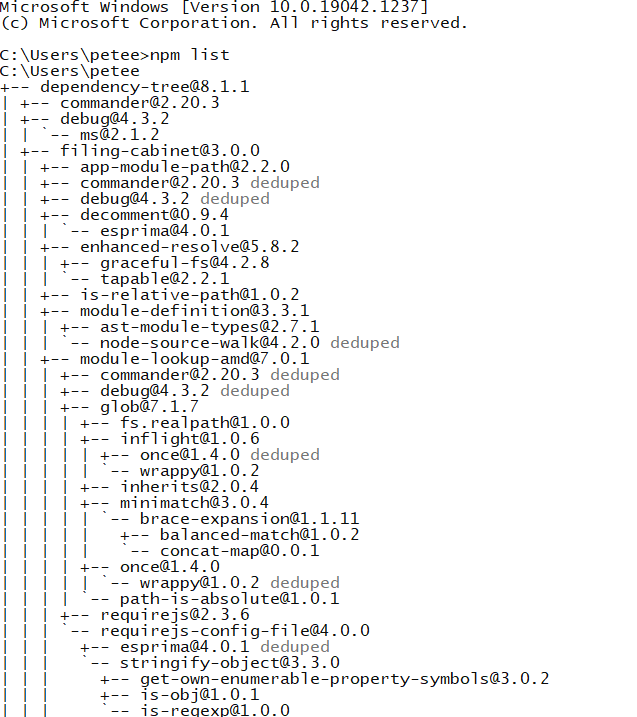
\includegraphics[scale=0.45]{images/npm_ls.png}
		\caption{npm list}
		\label{fig:npm-ls}
	\end{figure}
	
	\subsection{Dependency cruiser}
	
	A \textbf{Dependency cruiser} egy olyan szoftver, amely validálja és vizualizálja az adott csomag függőségeit, a felhasználó által megadott szabályok szerint.\\
	
	\textbf{Miért nem megfelelő}
	\begin{itemize}
		\item Alapvetően CLI-s használatra lett tervezve.
		\item Csak telepített csomagok esetében működik.
		\item Bár történik gráfkészítés, nem azon van a hangsúly.
		\item A gráf nagyobb projekteknél hatalmas, nem reprezentatív, nehezen betöltő \texttt{.svg} kiterjesztésű.
	\end{itemize}
	
	\begin{flushright}
		\cite{dep-cruise}
	\end{flushright}
	
	\begin{figure}[h]
		\centering
		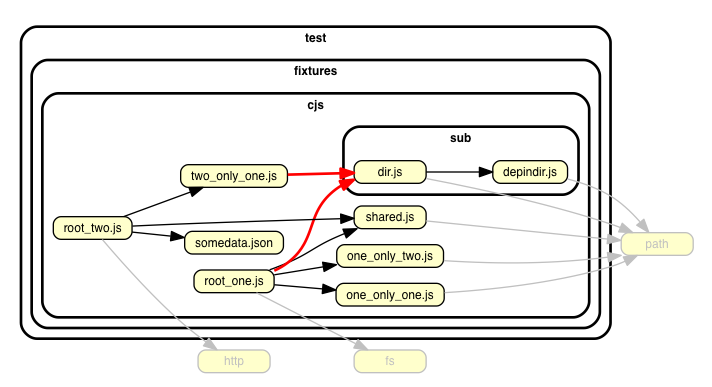
\includegraphics[scale=0.5]{images/dep_cruiser.png}
		\caption{Dependency cruiser}
		\label{fig:dep-cruiser}
	\end{figure}
	
	\subsection{Software Galaxies}
	
	A \textbf{Software Galaxies} egy olyan JavaScript alapú szoftver, amely képes vizualizálni olyan csomagkezelő rendszerek adatait, mint amilyen az npm is. Rendkívül látványos galaxisra emlékeztető 3 dimenziós objektumot hoz létre, mely a böngészőben jelenik meg és körbejárható. 
	
	Fejlesztése \textbf{Andrei Kashcha ("anvaka")} nevéhez fűződik.
	\\
	
	
	\textbf{Miért nem megfelelő}
	\begin{itemize}
		\item Rendkívül nagy a számításigénye.
		\item Inkább a csomagkezelőkön van a hangsúly, mint az npm csomagokon.
		\item Inkább érdekes és látványos (\ref{fig:sw-galaxies} ábra), mint hasznos.
	\end{itemize}
	
	\begin{flushright}
		\cite{anvaka-galaxies}
	\end{flushright}
	
	\begin{figure}[!h]
		\centering
		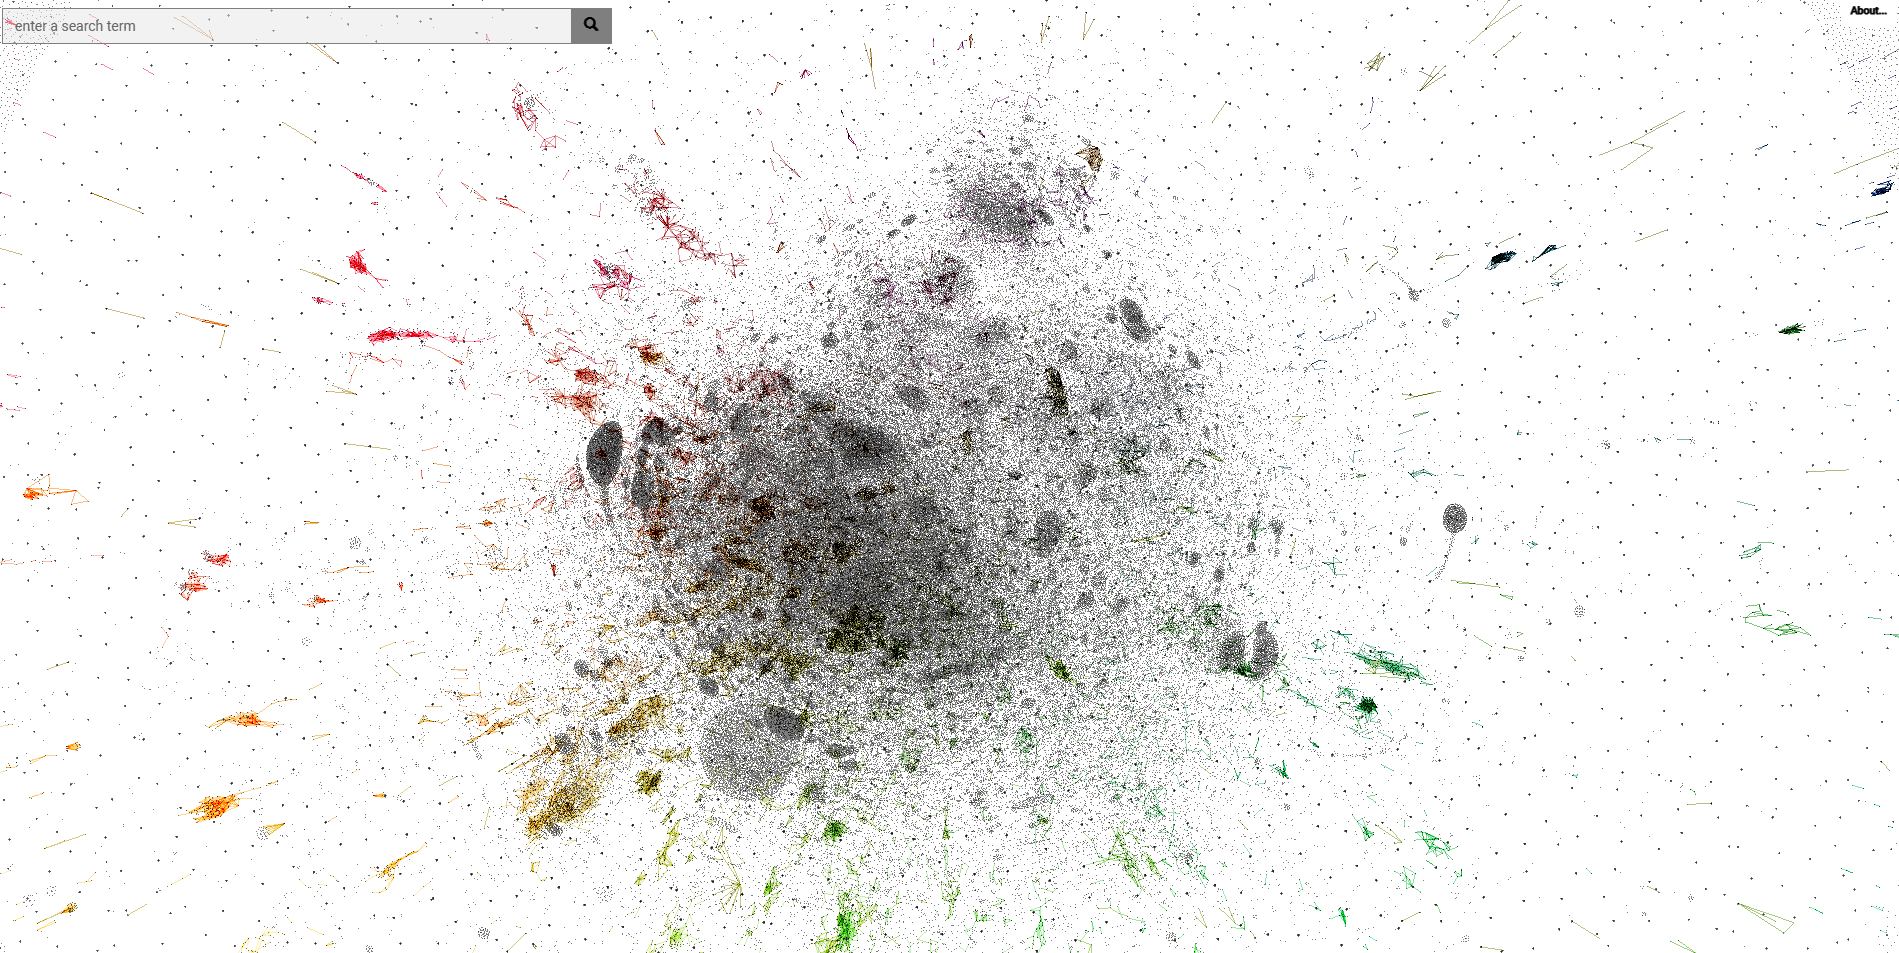
\includegraphics[scale=0.15]{images/anvaka_pm.png}
		\caption{Software Galaxies (Szín invertált)}
		\label{fig:sw-galaxies}
	\end{figure}
	
	\subsection{npmgraph.an}
	
	A \textbf{Software Galaxies} egy olyan JavaScript alapú szoftver, Angular.JS keretrendszert használó, interaktív webes szoftver, amely képes vizualizálni egy adott csomag függőségeit gráf formában. A kutatás során ez a szoftver állt a legközelebb az általam tervezett program jellegéhez.
	
	Fejlesztése szintén \textbf{Andrei Kashcha ("anvaka")} nevéhez fűződik.
	\\
	
	\textbf{Miért nem megfelelő:}
	\begin{itemize}
		\item A vizualizáció hálós gráfként történik, amely nem annyira informatív.
		\item Bár a gráfélek irányítottak célszerűbb nem látszik jól, ha esetleg valamilyen függőségi anomália van benne.
	\end{itemize}
	
	\textbf{Miért hasznos:}
	\begin{itemize}
		\item A megközelítés hasonló a vízióban felvázolthoz.
		\item Felvezeti a registry használatát.
	\end{itemize}
	
	\begin{flushright}
		\cite{anvaka-npmgraph}
	\end{flushright}
	
	\begin{figure}[!h]
		\centering
		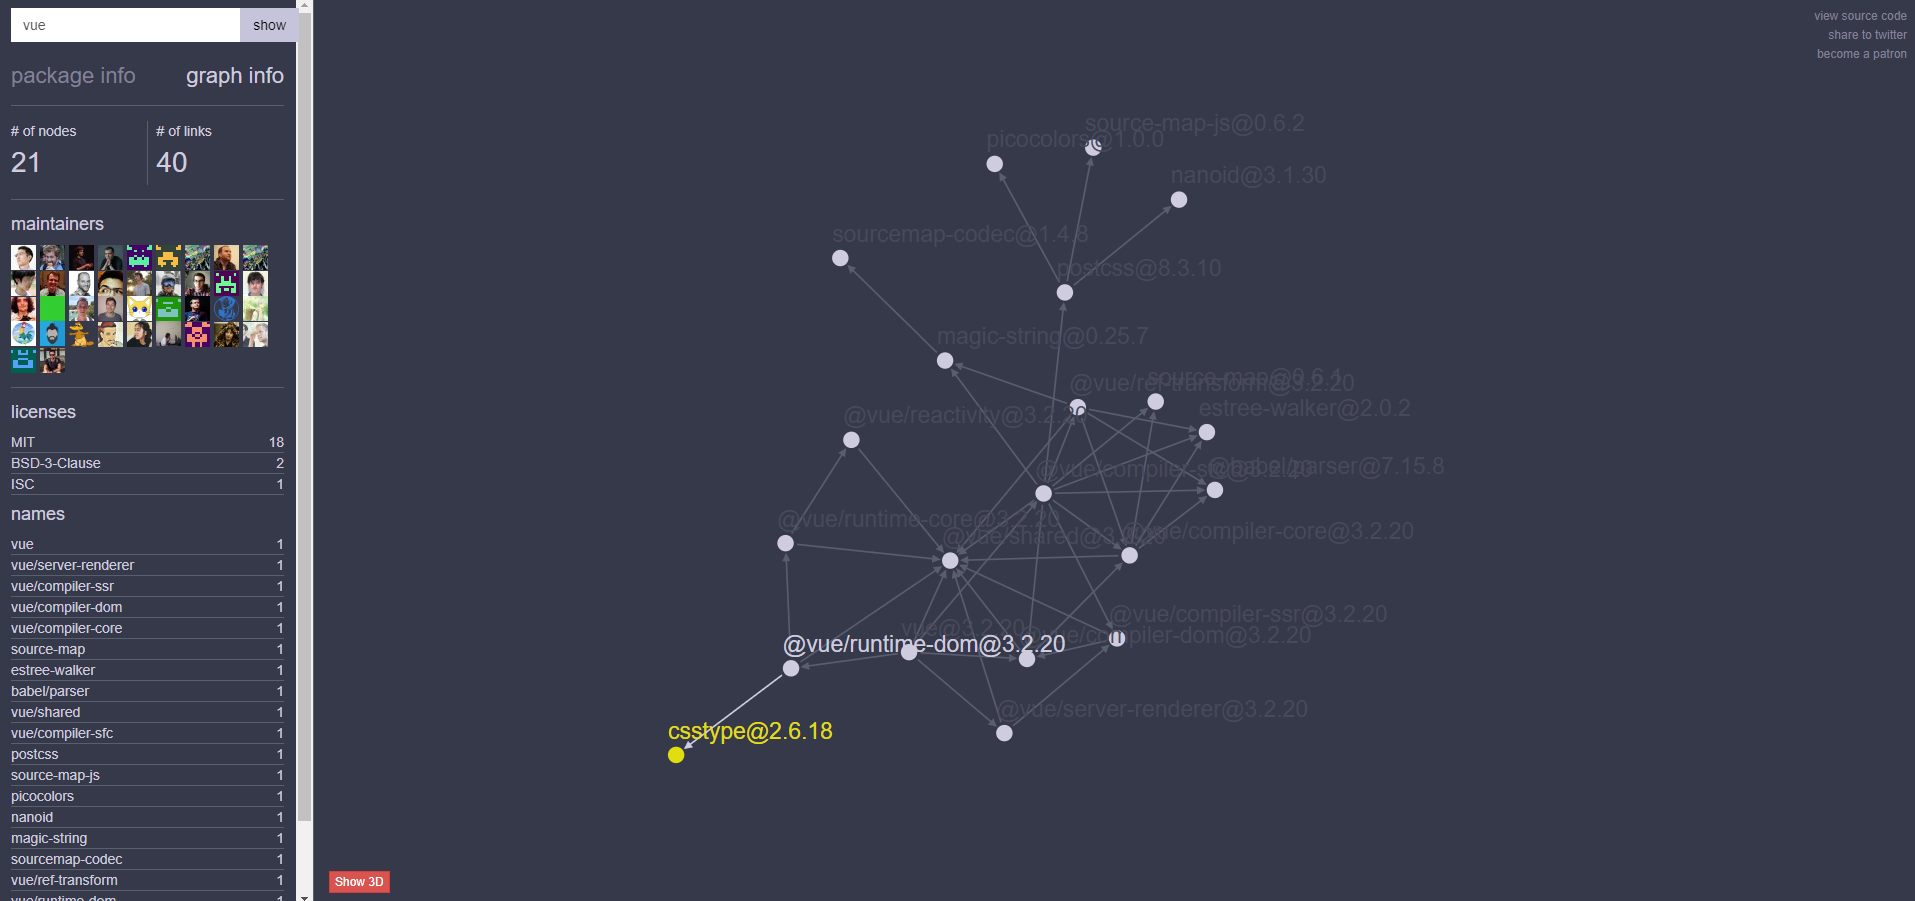
\includegraphics[scale=0.2]{images/anvaka_npmgraph.png}
		\caption{npmgraph.an}
		\label{fig:sw-npmgraph}
	\end{figure}
	
	\pagebreak

\section{Alkalmazott Technológiák}

A program megtervezésének következő lépése a technológiák, programozási nyelvek kiválasztása, amelyek szükségesek a megvalósításhoz.\\

Mivel a \hyperlink{section.2.2}{vízióban} meghatározásra került, hogy az alkalmazás egy web-applikáció lesz, így ez leszűkíti a kört a webes-technológiákra. Mivel a program az adatokat csak feldolgozni fogja, nem pedig tárolni, így se adatbázis, se API, tehát lényegében back-end sem szükséges, azaz egy front-end alkalmazás elkészítésére van szükség.\\

A felhasználói interfész lényegében a weboldal felülete lesz, amelynek testreszabása egyértelműen két jelölő nyelvet fog magával vonzzani:
\begin{itemize}
	\item HTML5
	\item CSS3
\end{itemize}

A jelölőnyelvekkel szép, áttekinthető UI hozható létre, azonban mivel nem programozási nyelvekről van szó, így szükség lesz egy olyan nyelvre is, amely a kliens oldalon szabályozza a weboldal működését. Mivel a legelterjedtebb és mindenhol általánosan elfogadott ilyen programnyelv a \textbf{JavaScript}, ezért erre esett a választás.\\

\textbf{Hasznos jellemzői:}
\begin{itemize}
	\item Magas-szintű nyelv
	\item Többszörös paradigma támogatás
	\item Futásidejű fordítás
	\item Prototípus alapú objektum orientáltság támogatása
\end{itemize}
\begin{flushright}
	\cite{javascript}
\end{flushright}

A JavaScript fontos jellemzője az említetteken kívül, hogy egy olyan programozási nyelv, amely az ECMAScript specifikációit követi. A legújabb ECMAScript verzió az ES12 (2021), azonban a legszéleskörűbb támogatást egyelőre az ES6 élvezi a böngészők nagy hányadánál. 

A JavaScript programok strukturálása a korai felhasználási módok miatt egy darabig abszolút nem volt létező fogalom, gyakorlatilag egy \texttt{.js} fájl tartalmazott minden javascript kódot, de volt rá precedens, hogy a html kódban a \texttt{<script></script>} tag-ek közé került a kód.

Bár mára a JavaScriptben lehetőség van funkciók, osztályok exportálására és importálására, ezt sokáig csak megkerülni tudták valamilyen más módszerrel.

Az npm-ben nagyon népszerű a \textbf{Babel}, egy olyan JavaScript fordító, amely képes az ES6+ veriójú JavaScript kódok ES5 verziójúra fordítani és futtatni.

A program megfelelő strukturálása, a téma és az esetlegesen hasznos csomagok miatt kényelmes megoldásnak bizonyul a programot egy \textbf{npm csomagként} megírni, illetve érdekességként a kész program képes lesz önmagát is elemezni.

A program funkcionalitása nem indokolja javascript keretrendszer szükségességét.

\pagebreak

\section{Tervezés}



